\documentclass[11pt,table]{beamer}
\mode<presentation>
\usepackage{etex}
\usepackage{graphicx}
\usepackage{epstopdf}
\usepackage[english]{babel}
\usepackage{tabularx}
\usepackage{booktabs}
\usepackage{mathrsfs}
\usepackage{multicol}
\usepackage{bm}
\usepackage{subcaption}
\usepackage{wrapfig}
\usepackage{dcolumn}
\usepackage{threeparttable}
\usepackage{booktabs}
\usepackage{bbm}
\usepackage{amsmath,dsfont,listings}
\usepackage{amssymb}
\usepackage{rotating}
\usepackage{multirow}
\usepackage{tcolorbox}
\usepackage[authoryear]{natbib}
\usepackage{circledsteps}
\usepackage{qtree}

\usepackage{tikz}
\usetikzlibrary{arrows,decorations.pathmorphing,backgrounds,fit,positioning,shapes.symbols,chains, shapes}
\setbeamertemplate{section in toc}[sections numbered]
\setbeamertemplate{caption}[numbered]

\bibliographystyle{Econometrica}

\setbeamersize{text margin right=3.5mm, text margin left=7.5mm}  % text margin
\setbeamersize{sidebar width left=0cm, sidebar width right=0mm}
\setbeamertemplate{sidebar right}{}
\setbeamertemplate{sidebar left}{}

\definecolor{text-grey}{rgb}{0.45, 0.45, 0.45} % grey text on white background
\definecolor{bg-grey}{rgb}{0.66, 0.65, 0.60} % grey background (for white text)
\definecolor{fu-blue}{RGB}{0, 51, 102} % blue text
\definecolor{fu-green}{RGB}{153, 204, 0} % green text
\definecolor{fu-red}{RGB}{204, 0, 0} % red text (used by \alert)
\definecolor{BrewerBlue}{HTML}{377EB8} % Define Brewer Blue
\definecolor{BrewerRed}{HTML}{E41A1C}  % Define Brewer Red
\definecolor{navy}{rgb}{0.0, 0.0, 0.5}
\definecolor{darkred}{HTML}{9c0404}

\setbeamertemplate{frametitle}{%
    \vskip-30pt \color{text-grey}\large%
    \begin{minipage}[b][23pt]{\textwidth}%
    \flushleft\insertframetitle%
    \end{minipage}%
}

\setbeamertemplate{navigation symbols}{} 

%%% begin title page
\setbeamertemplate{title page}{
\vskip2pt\hfill
\vskip19pt\hskip3pt

% set the title and the author
\vskip4pt
\parbox[top][1.35cm][c]{11cm}{\LARGE\color{text-grey} \textcolor{red1}{RL}earning:\\[1ex] \inserttitle \\[1ex] \small \quad \\[3ex]}
\vskip17pt
\parbox[top][1.35cm][c]{11cm}{\small Unit 2-2: \insertsubtitle \\[2ex] \insertauthor \\[1ex]}
}
%%% end title page

%%% colors
\usecolortheme{lily}
\setbeamercolor*{normal text}{fg=black,bg=white}
\setbeamercolor*{alerted text}{fg=fu-red}
\setbeamercolor*{example text}{fg=fu-green}
\setbeamercolor*{structure}{fg=fu-blue}

\setbeamercolor*{block title}{fg=white,bg=black!50}
\setbeamercolor*{block title alerted}{fg=white,bg=black!50}
\setbeamercolor*{block title example}{fg=white,bg=black!50}

\setbeamercolor*{block body}{bg=black!10}
\setbeamercolor*{block body alerted}{bg=black!10}
\setbeamercolor*{block body example}{bg=black!10}

\setbeamercolor{bibliography entry author}{fg=fu-blue}
\setbeamercolor{bibliography entry journal}{fg=text-grey}
\setbeamercolor{item}{fg=fu-blue}
\setbeamercolor{navigation symbols}{fg=text-grey,bg=bg-grey}
%%% end colors

%%% headline
\setbeamertemplate{headline}{
\vskip30pt
}
%%% end headline

%%% footline
\newcommand{\footlinetext}{
%\insertshortinstitute, \insertshorttitle, \insertshortdate
}
\setbeamertemplate{footline}{
\vskip2pt
\hfill \raisebox{-1pt}{\usebeamertemplate***{navigation symbols}}
\hfill \insertframenumber\hspace{10pt}
\vskip4pt
}
%%% end footline

%%% settings for listings package
\lstset{extendedchars=true, showstringspaces=false, basicstyle=\footnotesize\sffamily, tabsize=2, breaklines=true, breakindent=10pt, frame=l, columns=fullflexible}
\lstset{language=Java} % this sets the syntax highlighting
\lstset{mathescape=true} % this switches on $...$ substitution in code
% enables UTF-8 in source code:
\lstset{literate={ä}{{\"a}}1 {ö}{{\"o}}1 {ü}{{\"u}}1 {Ä}{{\"A}}1 {Ö}{{\"O}}1 {Ü}{{\"U}}1 {ß}{\ss}1}
%%% end listings

\usepackage{concmath}
\usepackage{xcolor}
\definecolor{red1}{RGB}{206, 17, 38}
\definecolor{blue1}{RGB}{16, 118, 208}
\definecolor{gray1}{RGB}{117, 115, 115}
\usepackage{hyperref}


\newtheorem{proposition}{Proposition}
\newtheorem{assumption}{Definition}

\title[]{Short guides to reinforcement learning}
\subtitle[]{Markov Decision Processes}
\author[D. Rostam-Afschar]{\textcolor{gray1}{Davud Rostam-Afschar (Uni Mannheim)}}
\date[]{\today}
\subject{Econometrics}
\renewcommand{\footlinetext}{\insertshortinstitute, \insertshorttitle, \insertshortdate}
\hypersetup{
    bookmarks=false,
    unicode=false,
    pdftoolbar=false,
    pdffitwindow=true,
    pdftitle={Reinforcement Learning for Business, Economics, and Social Sciences: \insertsubtitle},
    pdfauthor={Davud Rostam-Afschar},
    pdfsubject={Reinforcement Learning},
    pdfkeywords={reinforcement learning, Multi-Armed Bandits},
    pdfnewwindow=true,
}
\def\sym#1{\ifmmode^{#1}\else\(^{#1}\)\fi}

\begin{document}

\begin{frame}[plain]
  \titlepage
\end{frame}

% --------------------------------------------------- Slide --
%\begin{frame}
	%\frametitle{Content}
	%\tableofcontents[]
%\end{frame}

\section{Markov Decision Processes}
{
\setbeamercolor{background canvas}{bg=BrewerBlue}
\begin{frame}
\centering
\Huge
\textcolor{white}{How to take actions based on predictions?}
\thispagestyle{empty}
\end{frame}
}


\begin{frame}{Markov Decision Process}

    \begin{itemize}
        \item Markov process augmented with...

        \begin{itemize}
             
        
\item Actions e.g., $a_t$
\item Rewards e.g., $r_t$
    \end{itemize}
    \end{itemize}

\vspace{0.38cm} % Adjust this for vertical positioning

\begin{center}
\begin{tikzpicture}[
roundnode/.style={circle, draw=navy, thick, minimum size=7mm}]

% Nodes
\node[roundnode] (circle1) {$S_0$};
\node[roundnode] (circle2) [right=1.8cm of circle1] {$S_1$};
\node[roundnode] (circle3) [right=1.8cm of circle2] {$S_2$};
\node[roundnode] (circle4) [right=1.8cm of circle3] {$S_3$};
\node[roundnode] (circle5) [right=1.8cm of circle4] {$S_4$};

% Arrows
\draw[-latex, thick] (circle1.east) -- (circle2.west);
\draw[-latex, thick] (circle2.east) -- (circle3.west);
\draw[-latex, thick] (circle3.east) -- (circle4.west);
\draw[-latex, thick] (circle4.east) -- (circle5.west);

\end{tikzpicture}
\end{center}
    
\end{frame}

\begin{frame}{Markov Decision Process}

\vspace{-.8cm} % Adjust this for vertical positioning

    \begin{itemize}
        \item Markov process augmented with...

        \begin{itemize}
             
        
\item Actions e.g., $a_t$
\item Rewards e.g., $r_t$
    \end{itemize}
    \end{itemize}
		

\begin{center}
\begin{tikzpicture}[
roundnode/.style={circle, draw=navy, thick, minimum size=7mm},
squarenode/.style={rectangle, draw=darkred, thick, minimum width=7mm, minimum height=7mm}
]



% Nodes circles
\node[roundnode] (circle1) {$S_0$};
\node[roundnode] (circle2) [right=1.8cm of circle1] {$S_1$};
\node[roundnode] (circle3) [right=1.8cm of circle2] {$S_2$};
\node[roundnode] (circle4) [right=1.8cm of circle3] {$S_3$};
\node[roundnode] (circle5) [right=1.8cm of circle4] {$S_4$};

%Arrows (between circles)
\draw[-latex, thick] (circle1.east) -- (circle2.west) coordinate[midway] (arrow1);
\draw[-latex, thick] (circle2.east) -- (circle3.west) coordinate[midway] (arrow2);
\draw[-latex, thick] (circle3.east) -- (circle4.west) coordinate[midway] (arrow3);
\draw[-latex, thick] (circle4.east) -- (circle5.west) coordinate[midway] (arrow4);

% Nodes squares
\node[squarenode] (square1) [above=of arrow1] {$a_{0}$};
\node[squarenode] (square2) [above=of arrow2] {$a_{1}$};
\node[squarenode] (square3) [above=of arrow3] {$a_{2}$};
\node[squarenode] (square4) [above=of arrow4] {$a_{3}$};


%Arrows (between circles and square) up 

\draw[-latex, thick] (circle1.north east) -- (square1.west);
\draw[-latex, thick] (circle2.north east) -- (square2.west);
\draw[-latex, thick] (circle3.north east) -- (square3.west);
\draw[-latex, thick] (circle4.north east) -- (square4.west);

%Arrows (between circles and square) down 

\draw[-latex, thick] (square1.east) -- (circle2.north west);
\draw[-latex, thick] (square2.east) -- (circle3.north west);
\draw[-latex, thick] (square3.east) -- (circle4.north west);
\draw[-latex, thick] (square4.east) -- (circle5.north west);

\end{tikzpicture}
\end{center}
    
\end{frame}


\begin{frame}{Markov Decision Process}

\vspace{.3cm} % Adjust this for vertical positioning

    \begin{itemize}
        \item Markov process augmented with...

        \begin{itemize}
             
        
\item Actions e.g., $a_t$
\item Rewards e.g., $r_t$
    \end{itemize}
    \end{itemize}
\begin{center}
\begin{tikzpicture}[
roundnode/.style={circle, draw=navy, thick, minimum size=7mm},
squarenode/.style={rectangle, draw=darkred, thick, minimum width=7mm, minimum height=7mm},
diamondnode/.style={diamond, draw=darkred, thick, minimum size=7mm, text centered}
]



% Nodes circles
\node[roundnode] (circle1) {$S_0$};
\node[roundnode] (circle2) [right=1.8cm of circle1] {$S_1$};
\node[roundnode] (circle3) [right=1.8cm of circle2] {$S_2$};
\node[roundnode] (circle4) [right=1.8cm of circle3] {$S_3$};
\node[roundnode] (circle5) [right=1.8cm of circle4] {$S_4$};

%Arrows (between circles)
\draw[-latex, thick] (circle1.east) -- (circle2.west) coordinate[midway] (arrow1);
\draw[-latex, thick] (circle2.east) -- (circle3.west) coordinate[midway] (arrow2);
\draw[-latex, thick] (circle3.east) -- (circle4.west) coordinate[midway] (arrow3);
\draw[-latex, thick] (circle4.east) -- (circle5.west) coordinate[midway] (arrow4);

% Nodes squares
\node[squarenode] (square1) [above=of arrow1] {$a_{0}$};
\node[squarenode] (square2) [above=of arrow2] {$a_{1}$};
\node[squarenode] (square3) [above=of arrow3] {$a_{2}$};
\node[squarenode] (square4) [above=of arrow4] {$a_{3}$};


%Arrows (between circles and square) up 

\draw[-latex, thick] (circle1.north east) -- (square1.west);
\draw[-latex, thick] (circle2.north east) -- (square2.west);
\draw[-latex, thick] (circle3.north east) -- (square3.west);
\draw[-latex, thick] (circle4.north east) -- (square4.west);

%Arrows (between circles and squares) down 

\draw[-latex, thick] (square1.east) -- (circle2.north west);
\draw[-latex, thick] (square2.east) -- (circle3.north west);
\draw[-latex, thick] (square3.east) -- (circle4.north west);
\draw[-latex, thick] (square4.east) -- (circle5.north west);


% Nodes diamonds
\node[diamondnode] (diamond1) [below=of arrow1] {$r_{0}$};
\node[diamondnode] (diamond2) [below=of arrow2] {$r_{1}$};
\node[diamondnode] (diamond3) [below=of arrow3] {$r_{2}$};
\node[diamondnode] (diamond4) [below=of arrow4] {$r_{3}$};


%Arrows between diamonds and circles
\draw[-latex, thick] (circle1.south east) -- (diamond1.north);
\draw[-latex, thick] (circle2.south east) -- (diamond2.north);
\draw[-latex, thick] (circle3.south east) -- (diamond3.north);
\draw[-latex, thick] (circle4.south east) -- (diamond4.north);

%Arrows between diamonds and squares
\draw[-latex, thick] (square1.south) -- (diamond1.north);
\draw[-latex, thick] (square2.south) -- (diamond2.north);
\draw[-latex, thick] (square3.south) -- (diamond3.north);
\draw[-latex, thick] (square4.south) -- (diamond4.north);


\end{tikzpicture}
\end{center}
    
\end{frame}

\begin{frame}{Current Assumptions}

    \begin{itemize}
        \item Uncertainty: \textcolor{blue1}{stochastic} process
\item Time: \textcolor{blue1}{sequential} process
\item Observability: \textcolor{red1}{fully} observable states
\item No learning: \textcolor{red1}{complete} model
\item Variable type: \textcolor{red1}{discrete} (e.g., discrete states and  actions)

    \end{itemize}
\end{frame}

\begin{frame}{Markov Decision Process}

\begin{itemize}
    

\item  Definition

\begin{itemize}
     

\item Set of states: $\textcolor{red1}{S}$
\item Set of actions: $\textcolor{red1}{A}$
\item Transition model: $\textcolor{red1}{\mathbb{P}\left(s_{t} \mid s_{t-1}, a_{t-1}\right)}$
\item Reward model: $\textcolor{red1}{R\left(s_{t}, a_{t}\right)}$
\end{itemize}
\item  Goal: \textcolor{red1}{find optimal policy}
\end{itemize}

\vspace{5mm}
\footnotesize
 \textbf{Readings: Intro to Markov decision processes}\\
\citet[][chapter 3]{sutton2018reinforcement}
    
\citet[][chapter 2]{szepesvari2022algorithms}

\citet[][sections 17.1-17.2, 17.4]{russell2016artificial}
    
\citet[][chapters 2, 4, 5]{puterman2014markov}

\end{frame}


\section{(Discounted) Rewards and Values}
{
\setbeamercolor{background canvas}{bg=BrewerBlue}
\begin{frame}
\centering
\Huge
\textcolor{white}{(Discounted) Rewards and Values}
\thispagestyle{empty}
\end{frame}
}

\begin{frame}{What are the Rewards?}

\begin{itemize}
    \item \textbf{Rewards}: $r_{t} \in \mathbb{R}$


\item \textbf{Reward function}: $R\left(s_{t}, a_{t}\right)=r_{t}$ mapping from state-action pairs to rewards

\item Common assumption: \textcolor{red1}{stationary} reward function 

\begin{itemize}
\item $R\left(s_{t}, a_{t}\right)$ is the same $\forall t$
\end{itemize}
\item Exception: terminal reward function often different
\begin{itemize}
    
\item E.g., in a game: 0 reward at each turn and $+1 /-1$ at the end for winning/losing
\end{itemize}
\item Goal: \textbf{maximize sum of rewards} $\sum_{t} R\left(s_{t}, a_{t}\right)$
\end{itemize}
    
\end{frame}

\begin{frame}{Discounted Rewards}

\begin{itemize}
    \item If process infinite, isn't $\sum_{t} R\left(s_{t}, a_{t}\right)$ infinite?

\item Solution: \textcolor{red1}{discounted} rewards

\begin{itemize}
     

\item Discount factor: $0 \leq \gamma<1$
\item Finite utility: $\sum_{t} \gamma^{t} R\left(s_{t}, a_{t}\right)$ is a geometric sum

\item $\gamma$ induces an (per-period) time‐preference rate of $\frac{1}{\gamma}-1$
\item Intuition: prefer utility sooner than later
\end{itemize}
\end{itemize}  
\end{frame}


\begin{frame}{Markov Decision Process}

\begin{itemize}
    

\item Definition

\begin{itemize}
     

\item Set of states: $\textcolor{red1}{S}$
\item Set of actions: $\textcolor{red1}{A}$
\item Transition model: $\textcolor{red1}{\mathbb{P}\left(s_{t} \mid s_{t-1}, a_{t-1}\right)}$
\item Reward model: $\textcolor{red1}{R\left(s_{t}, a_{t}\right)}$
\item Discount factor: $\textcolor{red1}{0 \leq \gamma \leq 1}$
\begin{itemize}
\item discounted: $\gamma<1$
\item undiscounted: $\gamma=1$
\end{itemize}
\item Horizon (i.e., \# of time steps): $\textcolor{red1}{h}$
\begin{itemize}
\item Finite horizon: $h \in \mathbb{N}$
\item infinite horizon: $h=\infty$
\end{itemize}
\end{itemize}
\item  Goal: \textcolor{red1}{find optimal policy}
\end{itemize}

\end{frame}


\begin{frame}{Inventory Management}

\begin{columns}[T]
\begin{column}{0.6\textwidth}
\begin{itemize}
   \item Markov Decision Process
   \begin{itemize}
\item States: \textcolor{red1}{inventory levels}
\item Actions: \textcolor{red1}{\{doNothing, orderGoods\}}
\item Transition model: \textcolor{red1}{stochastic demand}
\item Reward model:\\ \textcolor{red1}{Sales - Costs - Storage}
\item Discount factor: \textcolor{red1}{0.999}
\item Horizon: $\textcolor{red1}{\infty}$
\end{itemize}
\end{itemize}
\end{column}
\begin{column}{0.4\textwidth}
\centering
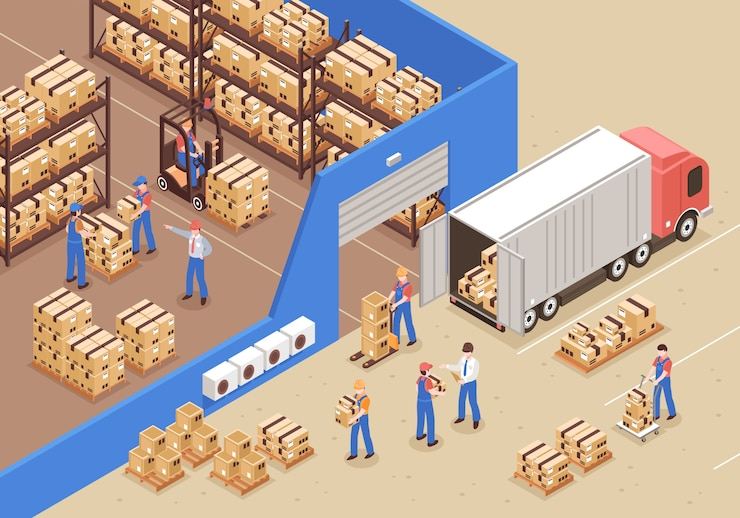
\includegraphics[width=0.9\textwidth]{figures/4.png}
\end{column}
\end{columns}
\vspace{5mm}
\begin{itemize}
    \item Tradeoff: \textcolor{red1}{increasing supplies decreases odds of  missed sales, but increases storage costs}
 \end{itemize}

\end{frame}



\section{Policies to Max Expected Utility}
{
\setbeamercolor{background canvas}{bg=BrewerBlue}
\begin{frame}
\centering
\Huge
\textcolor{white}{Policies to Max Expected Utility}
\thispagestyle{empty}
\end{frame}
}

\begin{frame}{What is a Policy?}

\begin{itemize}
    \item Choice of action at each time step

\item Formally:
\begin{itemize}
    \item Mapping from states to actions
\item i.e., $\pi(s_t)=a_t$
\item Assumption: \textcolor{red1}{fully observable states}
 \begin{itemize}
     \item Allows $a_t$ to be chosen only based on current state $s_t$
 \end{itemize}
\end{itemize}
 
\end{itemize}
    
\end{frame}



\begin{frame}{Policy Optimization}

\begin{itemize}
    \item Policy evaluation:
\begin{itemize}
     
 \item Compute expected utility
$$
V^{\pi}\left(s_{0}\right)=\sum_{t=0}^{h} \gamma^{t} \sum_{s_{0}} \mathbb{P}\left(s_{t} \mid ..., s_{0}, \pi\right) R\left(s_{t}, \pi\left(s_{t}\right)\right)
$$
\end{itemize}
\item Optimal policy:

\begin{itemize}
    \item Policy with highest expected utility

$$
V^{\pi^{*}}\left(s_{0}\right) \geq V^{\pi}\left(s_{0}\right) \forall \pi
$$ 
\end{itemize}
\end{itemize}
    
\end{frame}


\begin{frame}{Policy Optimization}

\begin{itemize}
    \item Several classes of algorithms:
\begin{itemize}
    \item \textcolor{red1}{Value iteration}
\item \textcolor{red1}{Policy iteration}
\item \textcolor{red1}{Linear programming}
\item \textcolor{red1}{Search techniques}
 
\end{itemize}

 \item Computation may be done


\begin{itemize}
    \item \textcolor{red1}{Offline}: before the process starts
\item \textcolor{red1}{Online}: as the process evolves
 
\end{itemize}
\end{itemize}
    
\end{frame}


\begin{frame}[t,allowframebreaks
]%\nocite{*}
\frametitle{References}
\small
\bibliography{bib}
\end{frame}
\section{Takeaways}
{
\setbeamercolor{background canvas}{bg=BrewerBlue}
\begin{frame}
\centering
\Huge
\textcolor{white}{Takeaways}
\thispagestyle{empty}
\end{frame}
}

\begin{frame}{How Can Agents Choose Actions to Maximize Expected Rewards?}

\begin{itemize}
    \item Markov Decision Processes (MDPs) extend Markov processes with actions and rewards
    \item Goal: Find a policy that maps states to actions to maximize expected cumulative rewards		
    \item Policies can be optimized via value iteration, policy iteration, or other algorithms
    \item Discounting helps handle infinite horizons and captures preference for earlier rewards
\end{itemize}
\end{frame}


\end{document}
